
The selection of producers among the pool of workers can be achieved for each ledger cycle using a randomised approach. Since a producer generates a ledger state update for a ledger cycle based on transactions collected during the previous ledger cycle(s), such assignment to a node should be revealed at least one cycle ahead. Assume that at the beginning of a ledger cycle $C_n$ at time $t = t_{n,0}$, a random number $r$ is drawn using the Merkel tree of the ledger state update produced one cycle ahead ($C_{n-1}$) as seed to the PRNG. The random number $r$ is used to define the list of workers selected to become producers for the next cycle $C_{n+1}$ in the following way: for each worker node with an identifier $Id_i$ we define the quantity $u_i = Id_i \oplus r$ where $\oplus$ is an XOR function (for binary-based modulus addition). The list of new identifiers $\{u_i \}_{i=1,...,N}$ ($N$ is the total number of nodes in the pool of worker) is sorted in ascending order and the first $P$ identifiers in that list correspond to the nodes selected to be producers for the cycle $C_{n+1}$.\\


In a large network, it can be anticipated that a large number of nodes have available resource to be used to manage the ledger database and try to join the pool of workers (which we can translate as a high demand for work).
The size of the pool of workers must however be determined by security as well as economic factors. Indeed, it must be profitable for a node to join the pool of workers. Said otherwise, the average number of tokens earned by a producer over a period of time should cover its operation cost. As there might be more nodes willing to work than required for the pool of workers, nodes may join a secondary pool, \textit{a.k.a} work queue, a wait to be called to join the pool of workers. In order for these nodes to join the pool of workers, there must be a mechanism that limit the time period during which a node can be a worker. The approach considered is to grant nodes joining the pool of worker a worker pass which is valid for a limited period of time. For security reasons explained in section~\ref{Sec:ConSec}, rather than defining a strict expiry time, we associate a decay time to the validity worker pass. Similarly to unstable nuclear elements the work pass has a 50\% chance to remain valid after the worker sits in the pool of workers for a period of time equal to the decay time. The decay time is not fixed over time but instead can very depending on the quality of work performed by the worker when selected to be a producer. It can also vary to account for the demand for work, \textit{i.e.} the length of the work queue, although a threshold is considered to mitigate the risk of a malicious entity (or group of entities) trying to simulate a highest demand for work than reality, as explained below.\\ 


The list of identifiers of nodes in the pool of workers can be maintained in a dynamic hash table of fixed length ($DHT_w$) distributed across the network. Such table also stores the decay time of each node worker pass. ADD FORMULA PROBABILITY.\\
At the end of a ledger cycle, nodes in the network can therefore deduce the list of worker passes which validity has expired. Nodes on the network can update the table, freeing some slots that can be occupied by the nodes sitting in the queue. \\

By providing proof of their available resource to the network, nodes can spontaneously candidate to become worker: they join the work queue. Every node on the network can store such proof alongside the node identifier in dynamic hash table ($DHT_q$). As nodes leave the pool of workers, nodes from the queue can join it. Assuming the list of identifiers sorted chronologically in $DHT_q$, a logic can be implemented such that nodes with identifiers at the top of the list are the first ones to access the pool of workers. However, such approach may facilitate Sybil-identity attack scenarios, however expensive, if an entity controls a large number nodes at the top of the work queue (at least equal to half the pool of worker size $N/2$) and frequently adds many nodes to the work queue such that the size of the work queue pool is large enough to create an impression of a large demand for work.\\

 The peer identification protocol on Catalyst network is designed to limit the number nodes on the same IP address entering a pool of nodes. In particular the Ipv4 address space is small and limits the ability of an entity to spin up multiple nodes on different IP addresses. There is an exponential cost associated to get the number of distinct Ipv4 addresses needed to have enough nodes in the work queue.
We nevertheless consider an alternative approach to define the dynamic of nodes leaving the work queue and joining the pool of workers that both prevents Sybil attack and incentivise nodes to join the work queue during periods of low demand for work. We define a ranking (or score) associated to nodes in the work queue such that the work queue is not concurrent. The ranking is chronological but instead depends on the volume or flux of nodes joining the queue during same allotted time period. Nodes wanting to join the work queue during a small window of time register to a tertiary queue. At the end of the time window, a fixed and limited number of nodes from the tertiary queue are randomly selected. These nodes are given a ranking drawn from a normal distribution centred around the current lower rank of the work queue, which means that some selected nodes may obtain a ranking higher than nodes currently at the bottom of the work queue. The rest of the nodes in the tertiary queue are given a lower ranking drawn from a normal distribution centred around a lower rank value shifted from the current lower rank of the work queue, the shift being inversely proportional to the volume of nodes in the tertiary queue. The rotation rate of nodes in the pool of workers then depends on the size of the work queue but only take into account the number of nodes with a ranking higher than a given threshold. 

\newpage
\begin{landscape}
\begin{figure}
    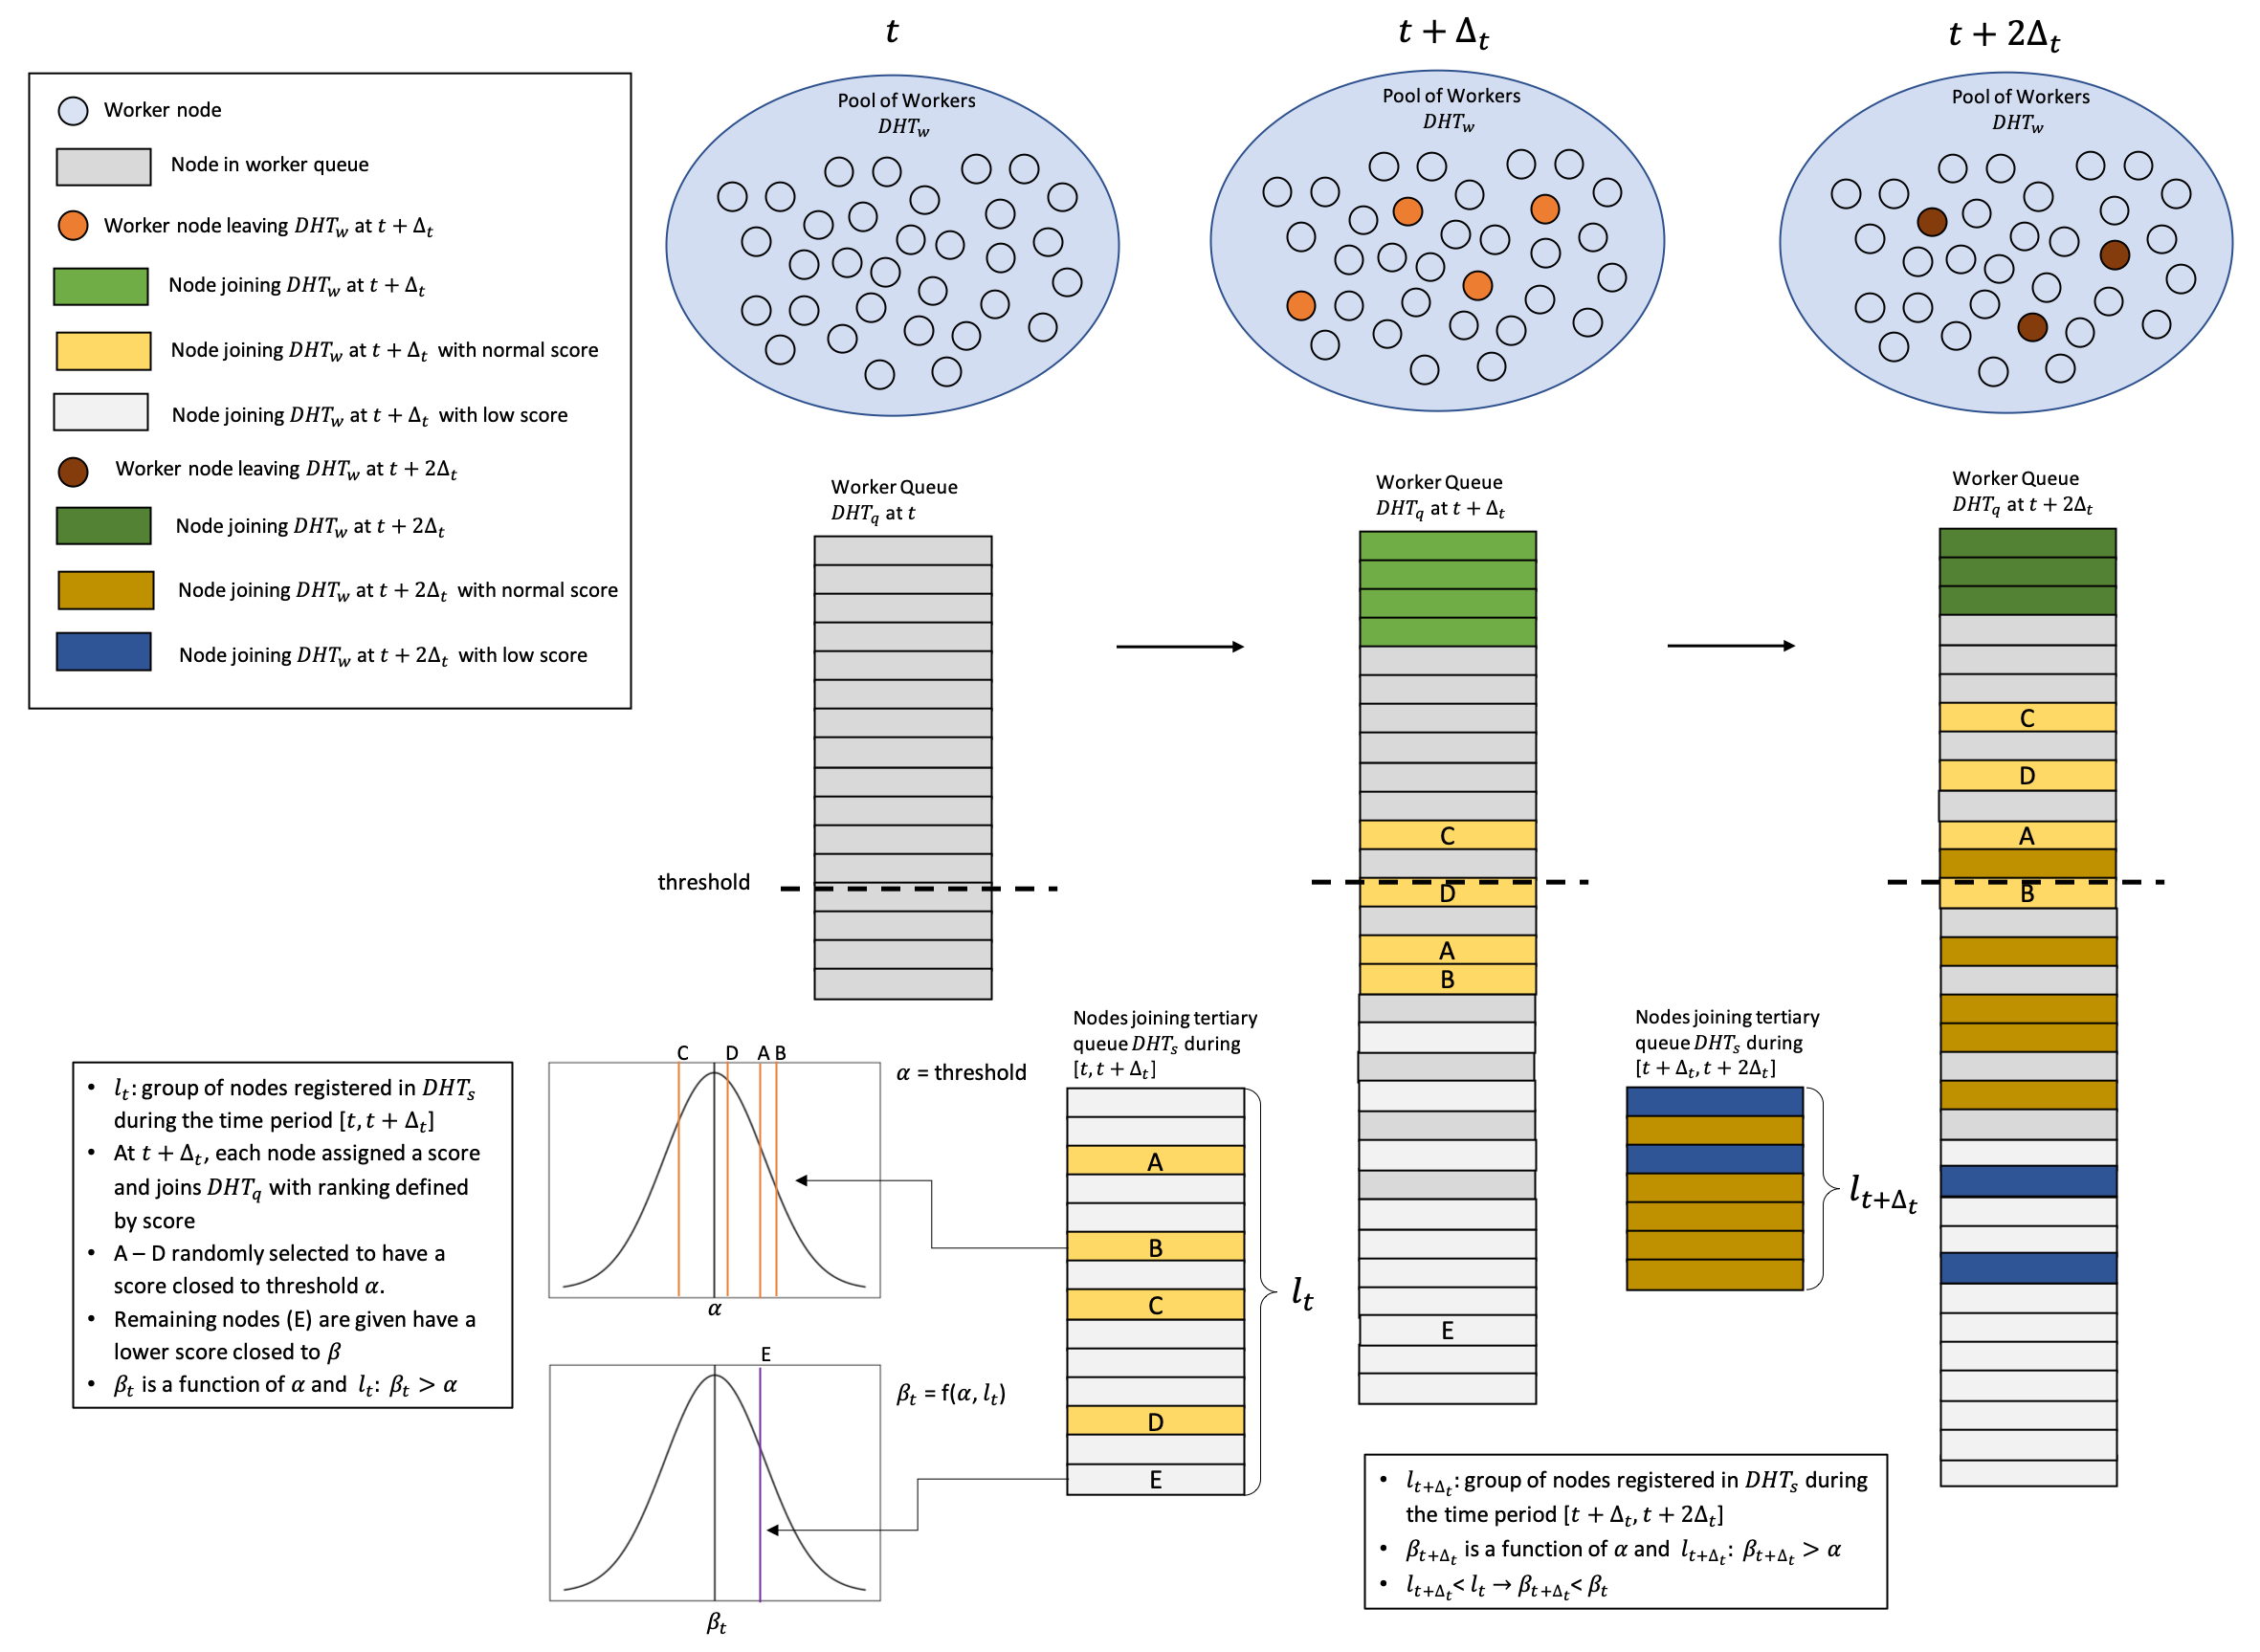
\includegraphics[width=22cm,height=42cm,keepaspectratio]{Figures/Work_Queue_Management}
    \caption{\label{fig:NSM}Illustration of the process followed by Catalyst network to add nodes to the work queue.}
\end{figure}
\end{landscape}

